
% Template for Elsevier CRC journal article
% version 1.2 dated 09 May 2011

% This file (c) 2009-2011 Elsevier Ltd.  Modifications may be freely made,
% provided the edited file is saved under a different name

% This file contains modifications for Procedia Computer Science
% but may easily be adapted to other journals

% Changes since version 1.1
% - added "procedia" option compliant with ecrc.sty version 1.2a
%   (makes the layout approximately the same as the Word CRC template)
% - added example for generating copyright line in abstract

%-----------------------------------------------------------------------------------

%% This template uses the elsarticle.cls document class and the extension package ecrc.sty
%% For full documentation on usage of elsarticle.cls, consult the documentation "elsdoc.pdf"
%% Further resources available at http://www.elsevier.com/latex

%-----------------------------------------------------------------------------------

%%%%%%%%%%%%%%%%%%%%%%%%%%%%%%%%%%%%%%%%%%%%%%%%%%%%%%%%%%%%%%
%%%%%%%%%%%%%%%%%%%%%%%%%%%%%%%%%%%%%%%%%%%%%%%%%%%%%%%%%%%%%%
%%                                                          %%
%% Important note on usage                                  %%
%% -----------------------                                  %%
%% This file should normally be compiled with PDFLaTeX      %%
%% Using standard LaTeX should work but may produce clashes %%
%%                                                          %%
%%%%%%%%%%%%%%%%%%%%%%%%%%%%%%%%%%%%%%%%%%%%%%%%%%%%%%%%%%%%%%
%%%%%%%%%%%%%%%%%%%%%%%%%%%%%%%%%%%%%%%%%%%%%%%%%%%%%%%%%%%%%%

%% The '3p' and 'times' class options of elsarticle are used for Elsevier CRC
%% Add the 'procedia' option to approximate to the Word template
%\documentclass[3p,times,procedia]{elsarticle}
\documentclass[3p,times]{elsarticle}

%% The `ecrc' package must be called to make the CRC functionality available
\usepackage{ecrc}
\usepackage{xcolor}

%% The ecrc package defines commands needed for running heads and logos.
%% For running heads, you can set the journal name, the volume, the starting page and the authors

%% set the volume if you know. Otherwise `00'
\volume{00}

%% set the starting page if not 1
\firstpage{1}

%% Give the name of the journal
\journalname{Procedia Computer Science}
\runauth{}
\jid{procs}

%% Give a short journal name for the dummy logo (if needed)
\jnltitlelogo{Procedia Computer Science}
\CopyrightLine{2011}{Published by Elsevier Ltd.}
%%%%%%%%%%%%%%%%%%%%%%%%%%%%%%%%%%%%%%%%%%%%%%%%%%%%%%%%%%%%%%%%%%%%%%%%%%

\usepackage{amssymb}
\usepackage[figuresright]{rotating}
\usepackage{float}
\usepackage{lscape}
\usepackage{xltabular}
\usepackage{array} 
\usepackage{tabularx}
\usepackage{ragged2e}
\usepackage{longtable}
\usepackage{geometry}
\usepackage{xltabular}

\usepackage{graphicx}
\usepackage{subcaption}
\usepackage[export]{adjustbox}
\usepackage{wrapfig}
\usepackage[rightcaption]{sidecap}
\usepackage{hyperref}

\begin{document}

\begin{frontmatter}

%% Title, authors and addresses

%% use the tnoteref command within \title for footnotes;
%% use the tnotetext command for the associated footnote;
%% use the fnref command within \author or \address for footnotes;
%% use the fntext command for the associated footnote;
%% use the corref command within \author for corresponding author footnotes;
%% use the cortext command for the associated footnote;
%% use the ead command for the email address,
%% and the form \ead[url] for the home page:
%%
%% \title{Title\tnoteref{label1}}
%% \tnotetext[label1]{}
%% \author{Name\corref{cor1}\fnref{label2}}
%% \ead{email address}
%% \ead[url]{home page}
%% \fntext[label2]{}
%% \cortext[cor1]{}
%% \address{Address\fnref{label3}}
%% \fntext[label3]{}

\dochead{}
%% Use \dochead if there is an article header, e.g. \dochead{Short communication}
%% \dochead can also be used to include a conference title, if directed by the editors
%% e.g. \dochead{17th International Conference on Dynamical Processes in Excited States of Solids}

\title{BlockEstate: Revolutionizing Real Estate Transactions through Hyperledger-Based Blockchain Technology}

%% use optional labels to link authors explicitly to addresses:
\author[label1]{Laviza Falak Naz}%
%\author[label1]{Author 2}
%\author[label2]{Author 3}
\address[label1]{NED University of Engineering \& Technology}
%\address[label2]{Affiliation 2}

\begin{abstract}
This paper presents BlockEstate, an innovative real estate transaction platform built on the Hyperledger blockchain framework. BlockEstate introduces a unique chaincode for property ownership management, coupled with a novel pay order mechanism, revolutionizing the traditional real estate transaction process. The platform leverages blockchain technology's decentralization, immutability, and transparency to address the prevalent inefficiencies and security concerns in real estate transactions. The chaincode automates property ownership transfer, while the pay order mechanism ensures secure and transparent financial transactions. This paper explores the architecture, functionality, and application of BlockEstate, including a detailed analysis of its security and privacy features, and examines the challenges and limitations inherent in implementing blockchain technology in the real estate sector. A hypothetical case study demonstrates the practical application of BlockEstate, highlighting its efficiency, security, and transformative potential in the real estate market. The paper concludes by discussing the future prospects of blockchain in real estate and the role of platforms like BlockEstate in shaping this future.
\end{abstract}

\begin{keyword}
%% keywords here, in the form: keyword \sep keyword
%% PACS codes here, in the form: \PACS code \sep code
%% MSC codes here, in the form: \MSC code \sep code
%% or \MSC[2008] code \sep code (2000 is the default)
Blockchain Technology \sep Real Estate Transactions \sep Hyperledger Framework \sep Chaincode \sep Property Ownership Management \sep Pay Order Mechanism \sep Decentralization \sep Transaction Security \sep Financial Transparency \sep Smart Contracts \sep Digital Tokenization \sep Property Token
\end{keyword}

\end{frontmatter}

%%
%% Start line numbering here if you want
%%
% \linenumbers

%% main text
\section{Introduction}

The advent of blockchain technology has ushered in a new era of innovation across various industries, with the real estate sector being no exception. Traditional real estate transactions are often hampered by lengthy procedures, lack of transparency, and high susceptibility to fraud \cite{saari2022blockchain}. These challenges necessitate a robust solution that streamlines transactions while ensuring security and transparency. This paper introduces BlockEstate, a pioneering real estate transaction platform built on the Hyperledger blockchain framework. BlockEstate leverages the inherent benefits of blockchain technology, such as decentralization, immutability, and transparency, to revolutionize real estate transactions \cite{garcia2020legal}. The platform employs a unique chaincode for property ownership management, underpinned by a novel pay order mechanism, which enhances the efficiency and security of property transactions.

BlockEstate’s architecture offers a comprehensive solution to the prevalent inefficiencies in the real estate sector. By enabling a decentralized ledger system, it ensures that all transactions are transparent and immutable. The platform’s chaincode is specifically designed to manage property ownership, while the pay order mechanism guarantees secure and transparent financial transactions between buyers and sellers \cite{ullah2023conceptual}. This paper aims to elucidate the functionality, benefits, and potential impact of BlockEstate in reforming real estate transactions.

\section{Related Work}

The integration of blockchain technology in real estate has been a subject of growing interest in recent academic and industry research \cite{podshivalov2022improving}. Several studies have highlighted the potential of blockchain in addressing the key challenges of real estate transactions, such as fraud, lack of transparency, and inefficiency \cite{wouda2019blockchain}. Blockchain’s attributes, notably its decentralized nature and tamper-proof ledger, have been identified as crucial in enhancing the trustworthiness and efficiency of real estate transactions \cite{latifi2019blockchain}.

Prior applications of blockchain in real estate primarily focused on digitizing property records and simplifying title transfers \cite{konashevych2020constraints}. However, these applications often lacked comprehensive solutions for transaction management and financial security, which are critical in real estate dealings. Recent developments have seen the introduction of smart contracts to automate transaction processes \cite{veuger2020dutch}, yet the complexity of real estate transactions, encompassing legal, financial, and regulatory aspects, calls for a more tailored solution \cite{jeong2021implementation}.

BlockEstate's approach, utilizing Hyperledger’s modular and versatile framework, represents a significant advancement in this domain \cite{mittal2020real}. Hyperledger’s ability to support private transactions and configurable consensus mechanisms makes it well-suited for real estate applications where privacy and efficiency are paramount \cite{gupta2020tokenization}. The platform’s chaincode for property ownership management offers a more nuanced and adaptable solution compared to traditional smart contracts, catering specifically to the multifaceted nature of real estate transactions \cite{huh2020verification}.

Furthermore, the pay order mechanism introduced by BlockEstate addresses a critical gap in existing blockchain real estate solutions \cite{pankratov2020blockchain}. While previous models provided a secure ledger for property records, they often overlooked the complexity of financial transactions in real estate. BlockEstate’s mediation ledger concept not only ensures the security of financial transactions but also provides a transparent and reversible transaction mechanism, enhancing buyer and seller confidence \cite{ahmad2021real}.

In summary, while blockchain technology has been explored in the context of real estate transactions, BlockEstate’s innovative use of Hyperledger and its unique pay order mechanism fill a significant gap in the current literature and practice \cite{nijland2019influence}. This paper seeks to demonstrate the practicality and effectiveness of BlockEstate in transforming real estate transactions, setting a new benchmark in the application of blockchain technology in the sector.

\section{BlockEstate Architecture}

BlockEstate is a groundbreaking real estate transaction platform built upon the robust and versatile framework of Hyperledger blockchain \cite{bhanushali2020blockchain}. The architecture of BlockEstate is designed to cater specifically to the nuances and complexities of real estate transactions, offering a solution that is secure, transparent, and efficient \cite{konashevych2020general}. At the core of BlockEstate's architecture lies its decentralized ledger, which allows for the immutable recording of property transactions, thereby enhancing trust and transparency in the process.

\subsection{Hyperledger Framework}
The choice of Hyperledger as the underlying technology for BlockEstate is pivotal to its functionality. Unlike public blockchains, Hyperledger offers a permissioned network environment, which is essential for maintaining privacy in real estate transactions. It supports the creation of private channels, allowing specific data to be shared only with authorized participants, a feature crucial for handling sensitive information in property deals \cite{krupa2019reshaping}.

\subsection{Network Structure}
The network structure of BlockEstate is composed of various nodes, each representing different stakeholders in the real estate market, such as buyers, sellers, financial institutions, and regulatory bodies \cite{ferreira2021blockchain}. These nodes participate in the consensus process, ensuring the validity and authenticity of transactions. The architecture also includes smart contracts or chaincode, which automate transaction processes and enforce the business rules set forth by BlockEstate \cite{hoxha2019study}.

\subsection{Chaincode for Property Ownership}
A significant aspect of the architecture is the chaincode developed for property ownership management. This chaincode acts as an automated intermediary, managing and verifying ownership transfers. It ensures that all property data is accurately recorded and maintained on the blockchain \cite{mehendale2019implications}. Additionally, the chaincode facilitates the execution of complex transactions, including property tokenization, which represents real estate assets digitally on the blockchain.


\begin{figure}[H]
    \centering
    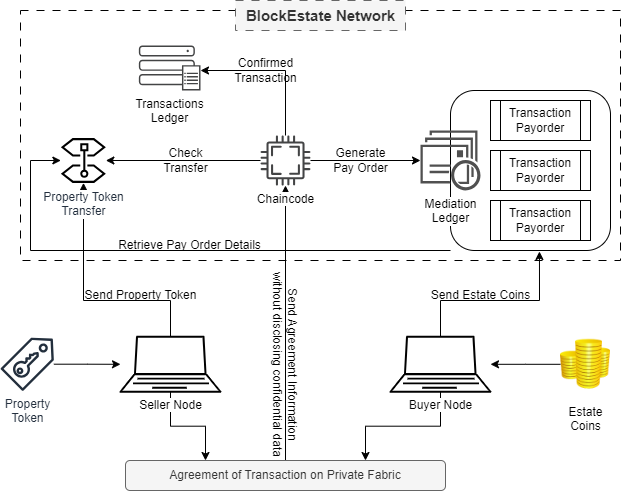
\includegraphics[width=1\linewidth]{images/Bllockchain.drawio.png}
    \caption{BlockEstate Architecture diagram}
    \label{fig:fig1}
\end{figure}

\section{Pay Order Mechanism}

The pay order mechanism in BlockEstate introduces an innovative approach to handling financial transactions within the real estate sector. This mechanism is integral to ensuring financial security and transparency in property transactions.

\subsection{Functionality}
When a property transaction is initiated, the buyer's funds are not directly transferred to the seller. Instead, they are placed into a mediation ledger in the form of a pay order. This ledger, accessible to all peers on the network, contains information about the transaction but restricts access to private data, which is only viewable by the buyer and seller \cite{avantaggiato2019challenges}.

\subsection{Security and Transparency}
The mediation ledger acts as a secure holding account for the transaction funds. It records all the transaction details while ensuring that the private information remains confidential. This process not only secures the funds but also provides transparency to all parties involved in the transaction \cite{sladic2021blockchain}.

\subsection{Automated Confirmation and Reversion}
The chaincode plays a crucial role in the pay order mechanism. Upon the transfer of the property token from the seller to the buyer, the chaincode automatically confirms the pay order in the mediation ledger and releases the funds to the seller. This automation ensures that the transfer of funds is contingent upon the successful transfer of property ownership \cite{mashatan2021usurping}. Conversely, if the property token is not transferred within the specified time period, the pay order is reverted, and the funds are returned to the buyer. This feature adds a layer of financial security, safeguarding the interests of both parties.

\begin{figure}[H]
    \centering
    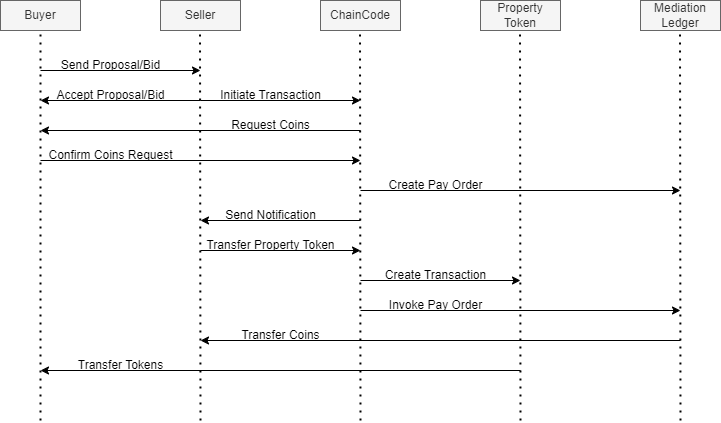
\includegraphics[width=1\linewidth]{images/state flow diagram.drawio.png}
    \caption{BlockEstate transaction flow diagram}
    \label{fig:fig2}
\end{figure}

In conclusion, the BlockEstate architecture, underpinned by the Hyperledger framework, and its innovative pay order mechanism collectively establish a new standard in real estate transactions. The integration of these technologies addresses many of the existing challenges in the real estate sector, offering a solution that is not only more efficient and secure but also transparent and user-friendly \cite{harris2021blockchain}.

\section{Chaincode Functionality}

The chaincode, a pivotal component of BlockEstate's architecture, serves as the backbone for the platform's transactional operations. It is essentially a set of programmable instructions executed on the Hyperledger blockchain, tailored to manage and facilitate real estate transactions.

\begin{verbatim}
Pseudocode for BlockEstate Chaincode

// Initialization of the chaincode
Initialize Chaincode
    Initialize ledger state

// Handler for various chaincode invocations
Invoke Function

// Create a new property record
CreateProperty(property details)
    Validate property details, Store property in ledger, Return success or error message

// Transfer property ownership
TransferProperty(property ID, new owner)
    Retrieve property from ledger, Verify ownership and transfer conditions, 
    Update property record with new owner, Return success or error message

// Create a pay order for a property transaction
CreatePayOrder(buyer, seller, amount)
    Validate transaction details, Create and store pay order in ledger, 
    Lock transaction amount in mediation ledger, Return success or error message

// Confirm a pay order upon successful property transfer
ConfirmPayOrder(pay order ID)
    Retrieve pay order from ledger, Verify property transfer completion,
    Update pay order status, Transfer funds from mediation ledger to seller, 
    Return success or error message

\end{verbatim}

\subsection{Technical Implementation}

The chaincode in BlockEstate is written in a high-level programming language, such as Go or JavaScript, which is supported by the Hyperledger Fabric framework. This programming model allows for the creation of sophisticated business logic to handle various aspects of property transactions \cite{veuger2020database}. The chaincode encapsulates the rules for property ownership transfer, pay order processing, and transaction validation.

\subsection{Property Ownership Management}

One of the primary functions of the chaincode is to manage property ownership records securely and efficiently. When a property is listed on the BlockEstate platform, the chaincode generates a unique digital token representing the property. This token contains essential details of the property, such as location, size, and legal information, securely stored on the blockchain  \cite{hermansson2020real}.

\subsection{Transaction Process Automation}

The chaincode automates the transaction process between buyers and sellers. When a transaction is initiated, the chaincode verifies the availability and ownership of the property token. It then oversees the pay order mechanism, ensuring that funds are securely held in the mediation ledger until all conditions of the sale are met \cite{saull2020can}.

\subsection{Ensuring Compliance and Security}

Through its programmable nature, the chaincode ensures that all transactions comply with predefined rules and regulations \cite{lindholm2021blockchain}. It also plays a crucial role in maintaining the security of the transactions, preventing unauthorized access and fraudulent activities.


\section{Case Study / Application Example}

To illustrate the practical application and benefits of BlockEstate, a hypothetical case study is presented.

\subsection{Background}

Consider a scenario where a buyer, Alice, is interested in purchasing a property from a seller, Bob. The property, located in a prime urban area, is listed on the BlockEstate platform \cite{li2019blockchain}.

\subsection{Initiation of Transaction}

Alice initiates the transaction on the BlockEstate platform. Upon her expression of interest, the chaincode generates a pay order, securing the transaction amount in the mediation ledger.

\subsection{Token Transfer and Pay Order Confirmation}

Bob transfers the property token to Alice using the BlockEstate platform. The chaincode verifies the transfer and automatically confirms the pay order. The funds from the mediation ledger are then released to Bob \cite{hutson2023architecting}.

\subsection{Efficiency and Security Benefits}

This case study demonstrates the efficiency and security benefits of BlockEstate. The transaction process is streamlined, reducing the time and complexity associated with traditional property transactions. Moreover, the security of funds and the transparency of the transaction are ensured through the chaincode and pay order mechanism \cite{bhatia2019exploration}.

\begin{figure}[H]
    \centering
    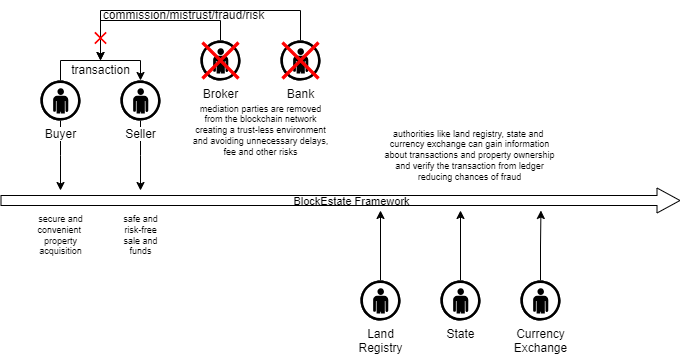
\includegraphics[width=1.0\linewidth]{images/use case.drawio.png}
    \caption{Application of BlockEstate Framework in Real Estate Market}
    \label{fig:fig3}
\end{figure}

In conclusion, the BlockEstate platform, through its innovative use of chaincode and the pay order mechanism, provides a more efficient, secure, and transparent method for real estate transactions, as exemplified in the case study.

\section{Security and Privacy Considerations}

The integration of blockchain technology in real estate transactions, as exemplified by BlockEstate, brings forth significant improvements in security and privacy. However, these advancements also necessitate a thorough examination of the associated risks and the measures taken to mitigate them \cite{kothari2020smart}.

\subsection{Data Encryption and Access Control}

In BlockEstate, sensitive data, including personal details of buyers and sellers and specifics of property tokens, are encrypted. The Hyperledger framework enables the implementation of sophisticated encryption methodologies to protect data at rest and in transit \cite{wu2023ebss}. Moreover, access control mechanisms are employed to ensure that only authorized participants have access to specific data, thereby safeguarding privacy.

\subsection{Smart Contract Security}

The chaincode, or smart contracts, in BlockEstate are rigorously tested to prevent vulnerabilities that could be exploited \cite{baum2021tokenization}. Regular audits and updates are part of the protocol to ensure the chaincode's integrity and security, thereby protecting the platform from potential breaches or fraudulent activities.

\subsection{Regulatory Compliance}

BlockEstate is designed to be compliant with existing real estate and data protection regulations \cite{moringiello2022blockchain}. The platform adheres to legal standards such as GDPR for data privacy and local real estate laws, ensuring that transactions are not only technologically secure but also legally sound.

\section{Challenges and Limitations}

Despite the innovative approach and advanced technology of BlockEstate, there are inherent challenges and limitations that need to be acknowledged \cite{tilbury2019business}.

\subsection{Technical Complexity}

The implementation of blockchain technology in real estate is technically complex. The development and maintenance of the BlockEstate platform require advanced technical expertise, particularly in blockchain technology and smart contract programming \cite{jain2020blockchain}. 

\subsection{Adoption and Integration}

The adoption of blockchain technology in the traditionally conservative real estate sector poses a significant challenge. Integrating BlockEstate with existing real estate processes and systems may encounter resistance and technical compatibility issues \cite{yacob2021blockchain}.

\subsection{Scalability and Performance}

As with many blockchain solutions, scalability and performance are potential limitations. Ensuring that BlockEstate can handle a large volume of transactions without compromising speed or efficiency is crucial for its long-term viability.

\section{Conclusion}

BlockEstate represents a significant advancement in the application of blockchain technology for real estate transactions. By leveraging the Hyperledger framework and implementing a unique pay order mechanism, BlockEstate addresses key challenges in the real estate sector, such as transaction inefficiency, lack of transparency, and security concerns.

The platform's innovative architecture and chaincode functionality bring a new level of efficiency, security, and transparency to real estate transactions \cite{shuaib2021improving}. While there are challenges and limitations, such as technical complexity and scalability concerns, the potential benefits of BlockEstate in revolutionizing real estate transactions are undeniable.

As blockchain technology continues to evolve, it is expected that solutions like BlockEstate will become increasingly sophisticated, overcoming current limitations and setting new standards in the real estate industry. The future of real estate transactions is poised for transformation, with BlockEstate at the forefront of this technological revolution.



\bibliographystyle{elsarticle-num}
\bibliography{references}

\end{document}